\documentclass[11pt,a4paper]{report}
\usepackage{titlesec}
\usepackage{listings}
\usepackage{graphicx}
\usepackage{wrapfig}
\usepackage[hidelinks]{hyperref}
\usepackage{tikz}
\usetikzlibrary{calc}
\usepackage[utf8]{inputenc}
\usepackage[left=3cm,right=3cm]{geometry}
\usepackage{calc}
\usepackage{eso-pic}
\usepackage{placeins}
\usepackage[document]{ragged2e}
\usepackage{titling}
\usepackage{float}

\begin{document}
    
\renewcommand\bibname{References}

\titleformat{\chapter}{\bfseries\huge\centering}{}{0pt}{}{\huge}
\titlespacing*{\chapter}{0pt}{-60pt}{40pt}
\setlength{\parindent}{2em}
\setlength{\parskip}{1em}

\newenvironment{myindentpar}[1]%
  {\begin{list}{}%
          {\setlength{\leftmargin}{#1}}%
          \item[]%
  }
  {\end{list}}

\title{Android Application Implementing ListView Using Linked List}

\author{Kashish Srivastava (185014)\\
        \and 
        Dipesh Kumar (185015)\\
        \and
        Akash Rana (185034)
}

\date{July 2020}



\pagestyle{plain}

\begin{titlepage}
    \begin{center}

        \Huge{\textbf{Android Application Implementing ListView Using Linked List}}
 
        \vspace{0.5cm}
        
        \normalsize
       
        \vspace{10pt}
        
    	Data Structures\\
        CSD-223

        
        
        \vspace{15pt}
        
\includegraphics[height=5cm]{./img/logo.png}
        
        \vspace{10pt}
        \textit{Submitted by:}

            Kashish Srivastava (185014)\\
            Dipesh Kumar (185015)\\
            Akash Rana (185034)
        \vspace{5pt}
        
        CSE (4 Year) : 
        4\textsuperscript{th} Semester
 
        \vspace{15pt}
 
        Under the guidance of
        
        \vspace{5pt}
        
        \textbf{Dr. Nitin Gupta }\\
        Assistant Professor, CSE Department\\
        National Institute of Technology, Hamirpur\\
 
        \vspace{25pt}
        
        \large
 
        Department of Computer Science and  Engineering\\
        National Institute of Technology, Hamirpur\\
      
    \end{center}
\end{titlepage}

\chapter{Abstract}		

Our goal was to develop a android application Implementing ListView using datastructure such as LinkedList. This Android application is basically coded in Kotlin. This Android application will provide our 
student and other people with the brief information of each and every department (i.e about different branches of engineering that are available in our institute) to have the better idea of every department of 
our institute and its courses available in that respective department. By developing this Android application, our basic idea was to provide the clear idea of how linked list, queue, stack and sets can be used 
to develop a well working an application.
\vspace{5pt} 


\tableofcontents

\chapter{Introduction}

The era of mobile technology opens the window to the android app development. The websites are vanishing and the mobile phones are emerging. It`s high time to changeform conventional form websites to apps, which 
has become the part of our daily routine. We are here introducing self made android application which would be a miniature part of our college website. It not only works as a website but also as a small college 
management software. This android application will provide our student and other managing staffs with the proper information of each and every department and of about its courses and placement. This android 
application is also a mobile version of the part of our institute official website.

This android application also uses different data structures in the development of the same. The data structures used in its development are linked list, queue, arrays, hash table etc. These all the data structure
 are pre provided by the android development for the development of such application.
 
 List view is used in this application to groups several items and display them in vertical scrollable list which is a list of department of our institute and similarly linked list is used in this application to 
 link last element with the recent one and also it allocates memory dynamically and hence these data structures are used in our application.

This project is basically designed to provide the better idea of how data structures i.e linked list,list view,hash table and arrays can be used to develop real life android application for the betterment of 
the coming youth.
\vskip 30cm



\chapter{Requirements and Installation}
	
The software and programming languages that are required to build an android application and we should also have prior knowledge about the following:-

\subsection*{\Large{Kotlin 1.32}}

Kotlin is a statically typed programming language for Java Virtual Machine (JVM) and JavaScript. Described as a general-purpose language, Kotlin introduces functional features to support Java
 interoperability. The Kotlin project was born out of the aspiration for heightened productivity. The goal was to improve the coding experience in a way that was both practical and effective.

\subsection*{\Large{Android Studio 3.6.1}}

Android Studio is an IDE, which is essentially an interface where you can enter your code (primarily Java or Kotlin) and access all the different tools necessary for development. 
Android Studio allows you to access libraries and APIs from the Android software development kit(SDK`s).

\subsection*{\Large{Android Virtual Device}}

An Android Virtual Device (AVD) is a configuration that defines the characteristics of an Android phone, tablet, Wear OS, Android TV, or Automotive OS device that you want to simulate in
 the Android Emulator. The AVD Manager is an interface you can launch from Android Studio that helps you create and manage AVDs.



 \chapter{Workflow and Components used}

The basic workflow to develop a working android application can be explained using the image given below:-
\begin{figure}[H]
	\centering
	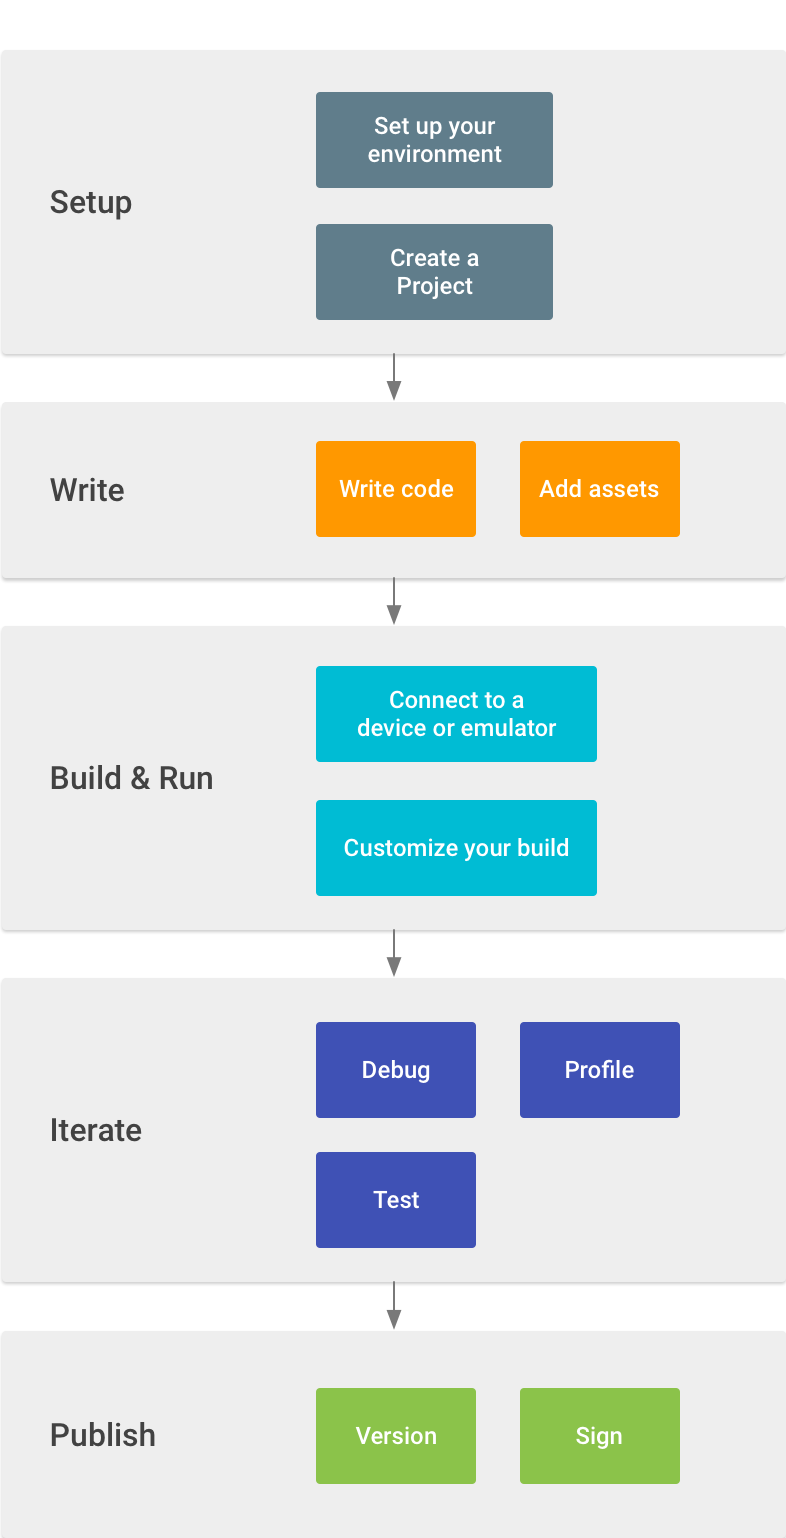
\includegraphics[scale=0.3]{./img/developer-workflow_2x.png}
	\caption{The workflow to develop an application .}
\end{figure}
\vskip 7cm



\textbf{{\large{Components used for Building the android application}}}
\section{ListView (View)}
\vskip 0.5cm
Android ListView is a view which contains the group of items and displays in a scrollable list. ListView is implemented by importing android.widget.ListView class. 
ListView is a default scrollable which does not use other scroll view.

ListView uses Adapter classes which add the content from data source (such as string array, array, database etc) to ListView. Adapter
 bridges data between an AdapterViews and other Views (ListView, ScrollView etc).

\begin{figure}[H]
	\centering
	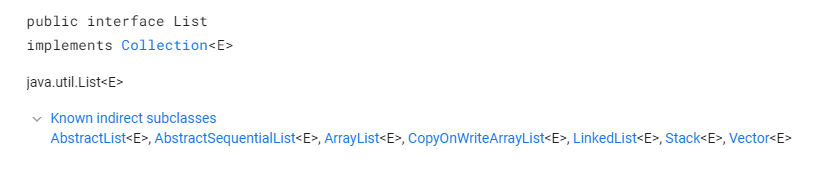
\includegraphics[scale=0.75]{./img/Screenshot (146).png}
\end{figure}


\section{Linked List (Data Structure)}
Doubly-linked list implementation of the List and Deque interfaces. Implements all optional list operations, and permits all elements (including null).

All of the operations perform as could be expected for a doubly-linked list. Operations that index into the list will traverse the list from the beginning or the end, whichever is closer to the specified index.
	\begin{figure}[H]
		\centering
    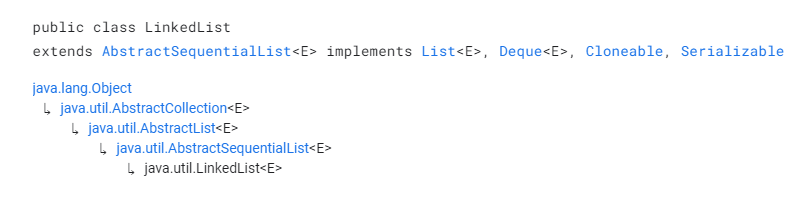
\includegraphics[scale=0.75]{./img/Screenshot (145).png}
  
	\end{figure}



\chapter{ListView Layout Design}

The display of elements in a list is a very common pattern in mobile applications. The user sees a list of items and can scroll through them. 
Typically the user interacts with the list via the toolbar, for example, via a button which refreshes the list. Individual list items can be selected. This selection can update the toolbar or can trigger a detailed screen for the selection. 


Every line in the widget displaying the data consists of a layout which can be as complex as you want. A typical line in a list has an image on the left side and two text lines in the middle as we have used here.
With Department picture on the left and Name of Department centered on the right.

\vspace{15pt}

\begin{figure}[H]
	\centering
		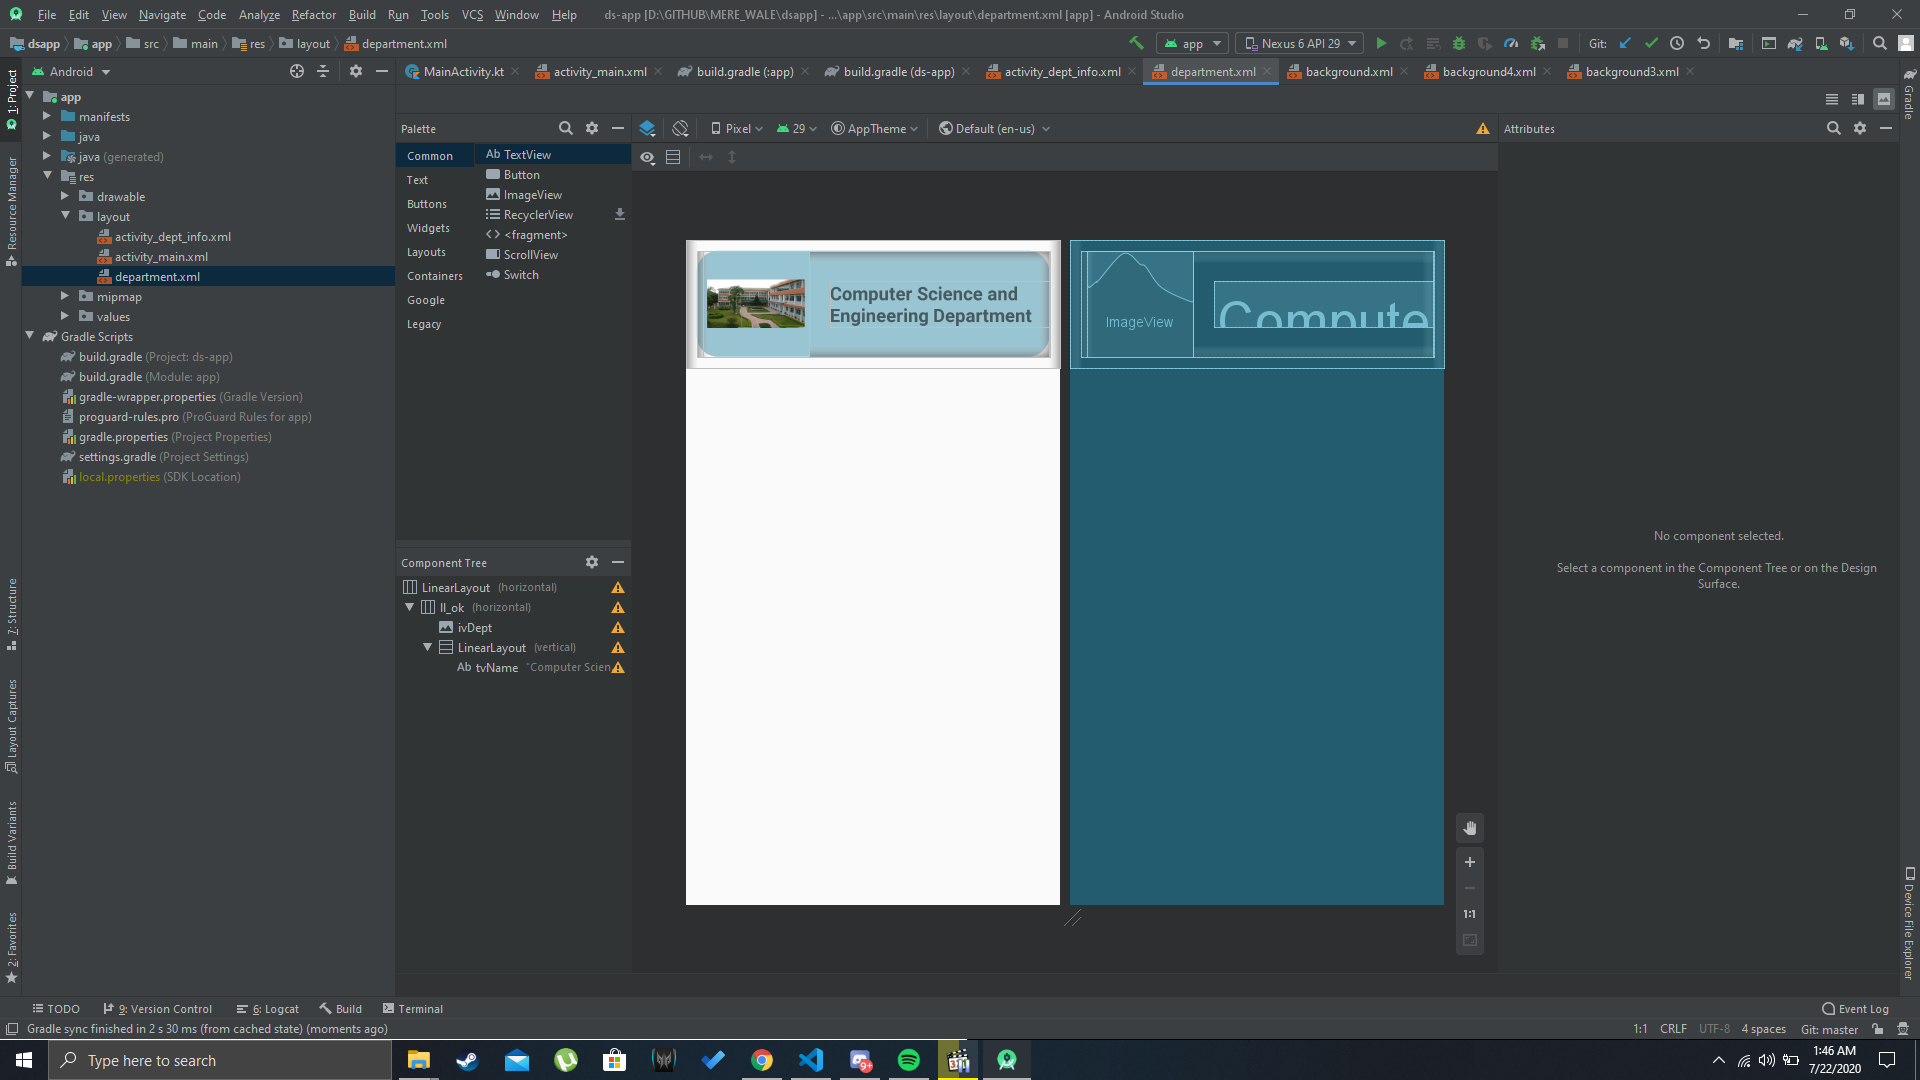
\includegraphics[scale=0.2]{./img/listview_2.png}
  \end{figure}

  \vspace{5pt}

We have to design the layout only once as this layout will be used for every item on the ListView.
This the crucial step as without designing a layout we wont be able to display the view 
anywhere , say activity\_main.xml layout or any other layout for that matter




\chapter{Load ListView with data using LinkedList}

Now, that the Layout for ListView has been created ,it needs to be populated with data.
In order to do this we use LinkedList.
First ,LinkedList is loaded with all the data that needs to be ported to ListView like we have
below in the LinkedList named ListOfDept.

\vspace{15pt}

\begin{figure}[H]
	\centering
		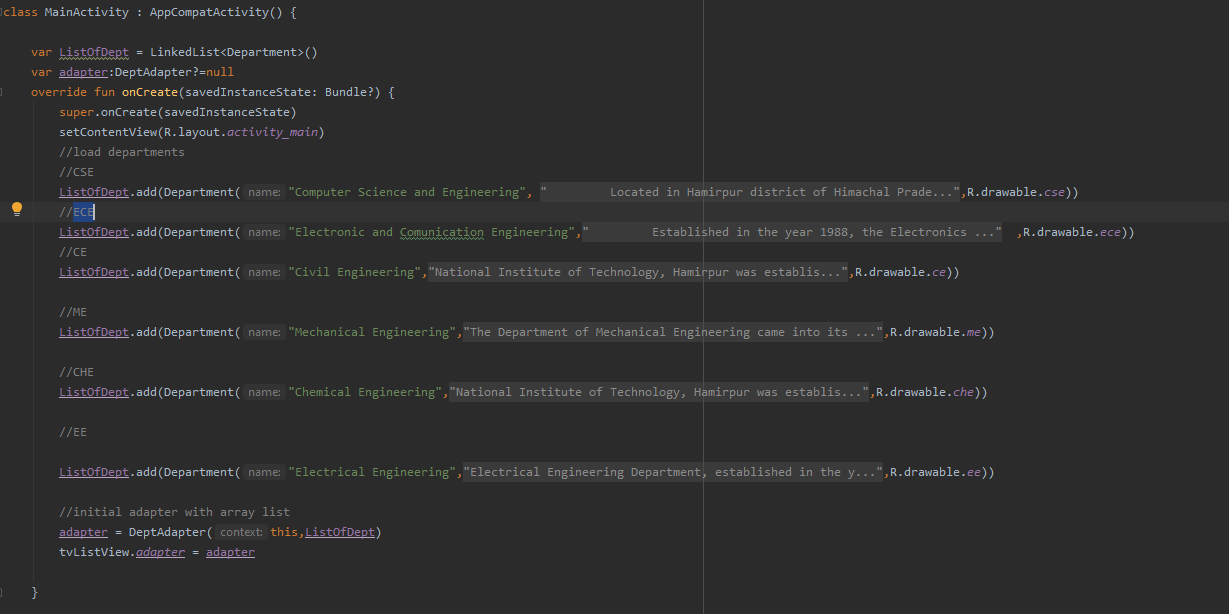
\includegraphics[scale=0.5]{./img/load_linked.PNG}
  \end{figure}

  \vspace{5pt}


After that we need to declare and implement our custom Adapter .An adapter manages the data model and adapts it to the individual entries in the widget. An adapter extends the BaseAdapter class.
The adapter would inflate the layout for each row in its getView() method and assign the data to the individual views in the row.
The adapter is assigned to the ListView via the setAdapter method on the ListView object.


\vspace{15pt}

\begin{figure}[H]
	\centering
		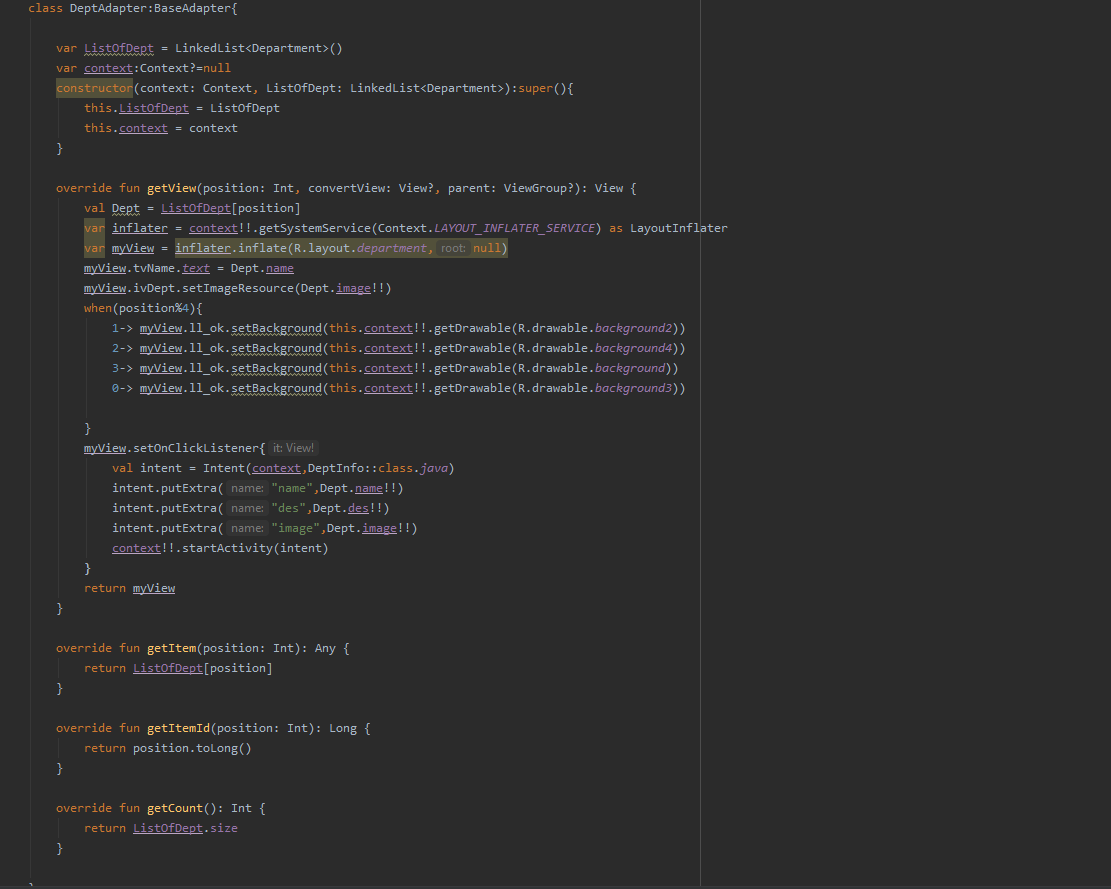
\includegraphics[scale=0.5]{./img/adapter.PNG}
  \end{figure}

  \vspace{5pt}

Main 2 functions in our adapter are  getView() and getCount().
getCount() returns the size of LinkedList which will be used in getView() func 
with ultimately return us view.
We have customized getView() function to return every element in list with different
background.
And a setOnClickListener has been setup to take us to another activity which gives detail 
about that particular department.


\chapter{ListView events}

After populating ListView with LinkedList data using our custom Adapter , new activity needs
to be created in order so that on clicking an item in ListView we are taken to Details about
that Department.

\vspace{15pt}
\begin{lstlisting}[ caption=setOnClickListener example]
myView.setOnClickListener{
    val intent = Intent(context,DeptInfo::class.java)
    intent.putExtra("name",Dept.name!!)
    intent.putExtra("des",Dept.des!!)
    intent.putExtra("image",Dept.image!!)
    context!!.startActivity(intent)
}

\end{lstlisting}

Here we have and example of such event which is triggered on clicking on an element of ListView.

Other than that we need to create a new activity and a layout.
The new layout we create must contain the picture of department , name and description
of the Department.
We use Constraint we rather than using LinearLayout that we used to wrap the listview.
Our new Layout looks something like this.


\vspace{15pt}

\begin{figure}[H]
	\centering
		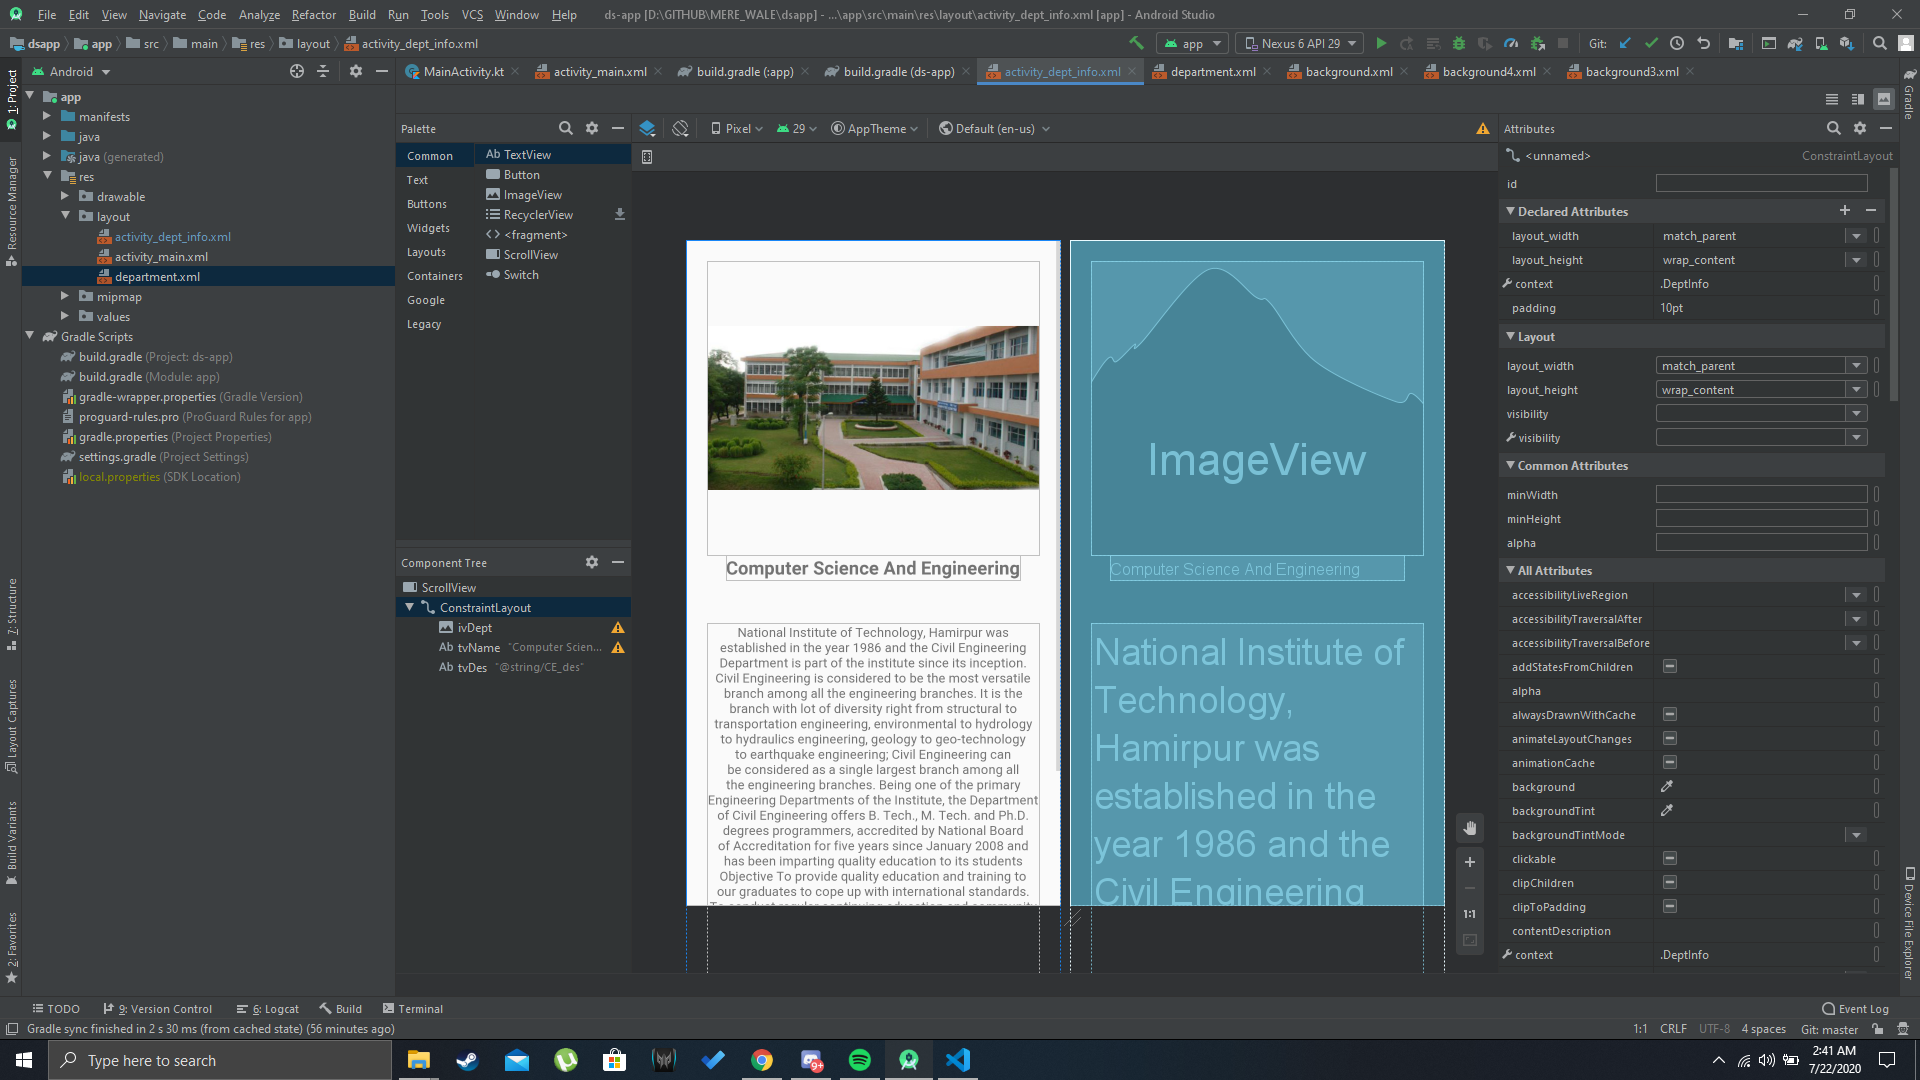
\includegraphics[scale=0.2]{./img/new_act.png}
  \end{figure}

  \vspace{5pt}


  Last thing required to implement is a new activity that is linked to the new layout we just 
  created.
  In the new activity we will provide the Name,description and the image of department which 
  will be given to the Layout.

  \begin{figure}[H]
    \centering
      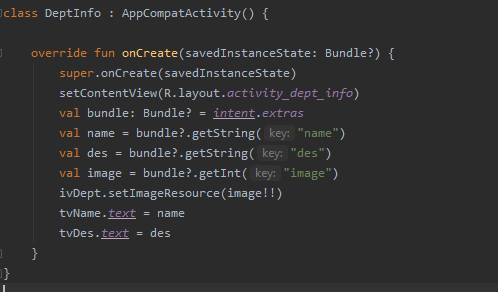
\includegraphics[scale=0.7]{./img/act.PNG}
    \end{figure}
  
    \vspace{5pt}

  All the Components required for the app are successfully implemented .
  Now we can just compile the whole code and used an AVD(Android Virtual Device)
  to view the finished application . We can also build the app as apk and use on an 
  actual android device. Built app will look something like:

  \begin{figure}[H]
    \centering
    \begin{minipage}[b]{0.3\textwidth}
      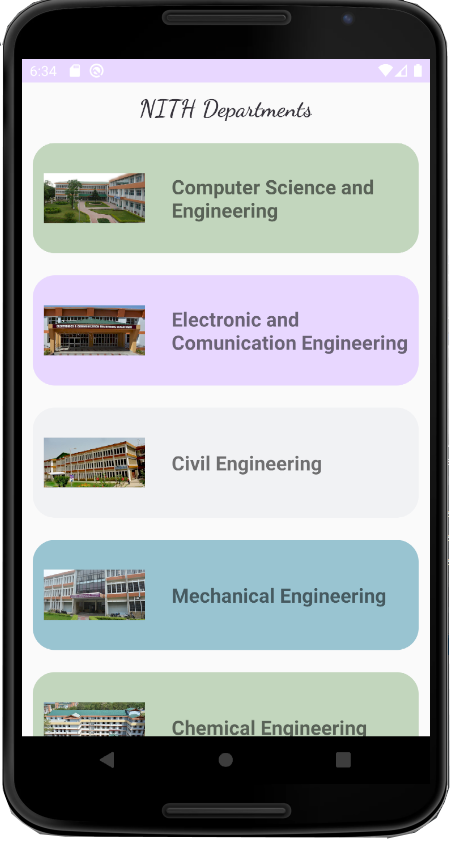
\includegraphics[width=\textwidth]{./img/PREVIEW1.png}
      \caption{activity\_main}
    \end{minipage}
    \hfill
    \begin{minipage}[b]{0.3\textwidth}
      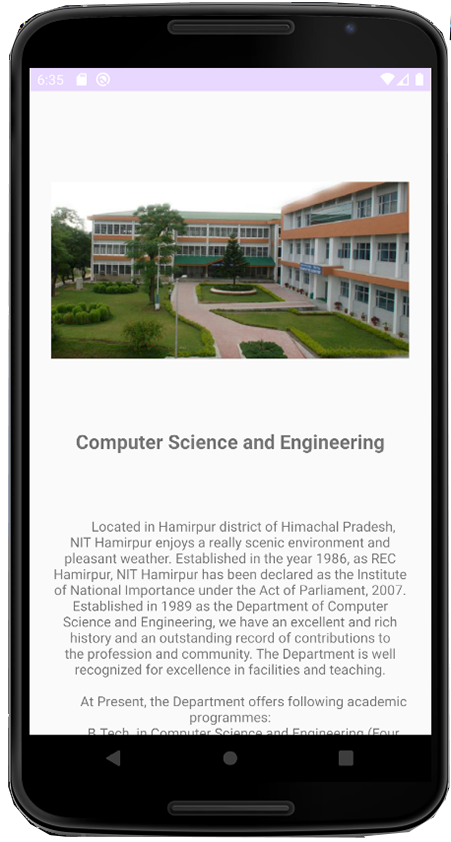
\includegraphics[width=\textwidth]{./img/PREVIEW2.png}
      \caption{activity\_dept\_info}
    \end{minipage}
  \end{figure}


\chapter{Conclusion}

This Project was a great opportunity for us to discover new fields and ways of working.
We have successfully implemented ListView with LinkedList in an android application.
LinkedList provides us with efficient form of storing data which needs to be retrieved
sequentially and ListView provides us with the ability to dynamically create lists 
with  custom layouts and with functionality of incepting tasks(such as opening a new activity) on clicking on a list item.

All these Components combined provide us with an effective android application that displays
the description of various departments of Engineering in National Institute of Technology
Hamirpur.



\chapter{References}
\vskip 1cm
{\large{The source code and other files related to this project can  be found at}\\
\url{https://github.com/cannibalcheeseburger/ds-app.git}\\
\vskip 1cm
\large{We used following references while working with this project:-}
\begin{itemize}
	\item  Natarajan Raman, Eunice Adutwumwaa Obugyei, Learning Kotlin by Building Android Applications: Explore the Fundamentals of Kotlin by Building Real-world Android Applications.
	\item Samuel Urbanowicz: Kotlin Standard Library Cookbook.
	\item \url{https://youtu.be/PJ3RdfJ4Np8}
	\item \url{http://developer.android.com/reference/packages.html}
	\item \url{http://developer.android.com/guide/topics/ui/index.html}
\end{itemize}
}

\end{document}